\documentclass[preprint,12pt]{elsarticle}
\usepackage{amsmath,amssymb,bm}
\usepackage{booktabs,multirow,threeparttable}
\usepackage{graphicx,subcaption}
\usepackage{siunitx}
\usepackage{xcolor}
\usepackage{hyperref}
\usepackage{lineno}
\usepackage{enumitem}
\usepackage{microtype}
\usepackage{placeins}
\emergencystretch=2em
\graphicspath{{../figures/}}
\hypersetup{colorlinks=true,linkcolor=blue!50!black,citecolor=blue!50!black,urlcolor=blue!60!black}
\journal{Transportation Research Part C}
\newcommand{\CNY}{\mathrm{RMB}}
\newcommand{\IJS}{\mathrm{IJS}}
\newcommand{\JS}{\mathrm{JS}}

\begin{document}
\begin{frontmatter}

\title{Data-driven collaborative optimization of three-dimensional highway alignments for life-cycle cost and mixed fuel--electric traffic energy}

\author[aff1]{Anonymous Author(s)}
\affiliation[aff1]{organization={Anonymous institution for double-anonymized review},
  city={Anonymous}, country={China}}

\begin{abstract}
Highway alignment couples plan geometry, profile, terrain, structures, urban development and long-term vehicle operation. We develop a spatially explicit bi-objective framework combining a quasi-natural digital elevation model, OpenStreetMap transport, water and buildings, and 14,018 GNSS points. Fifty plan modes and 224 referenced grade genes are searched collaboratively; centering leaves at most 223 locally independent grade degrees of freedom. Life-cycle cost includes land, basic works, structures, earthwork and maintenance, while the second objective monetizes 30-year fuel and electricity use for a mixed fleet. Spatial intersections trigger bridges, a connected mountain zone triggers ecological tunnelling, and dense cores are excluded. Improved Jellyfish Search approximates a weighted-sum front; feasibility, budget and non-dominance gates precede entropy-based selection.

The 22.46-km Guangzhou North Ring case anchors endpoint elevations, activates density constraints and uses spectral width $W=500$ m. The selected alignment reduces cost from 2.6406 to 2.4208 billion RMB (8.33\%) and energy cost from 1.3946 to 1.3528 billion RMB (3.00\%), with a 421-m minimum radius, zero hard penalty and no Tier-2 exposure. Tier-1 exposure falls from 2.010 to 1.591 km. The route is 12 m longer and uses more earthwork, but structure cost falls by 237 million RMB, exposing a physical trade-off rather than a length artefact. Earlier free-endpoint, unequal-budget experiments remain exploratory; current-model multi-seed, equal-NFE replication is required before design-grade use.
\end{abstract}

\begin{keyword}
highway alignment optimization \sep digital elevation model \sep OpenStreetMap \sep improved Jellyfish Search \sep life-cycle cost \sep mixed traffic energy \sep horizontal--vertical coordination
\end{keyword}
\end{frontmatter}

\linenumbers

\section{Introduction}

Highway alignment is an early design decision with long-lived consequences. A small lateral shift changes the terrain crossed, land take, bridge and tunnel demand, earthwork balance, maintenance exposure and the grades experienced by vehicles. These effects are coupled: shortening a horizontal path may worsen the vertical profile; avoiding a mountain may enter a dense urban zone; lowering earthwork can require a bridge; and a profile that appears energy-efficient in one direction can become infeasible at its network tie-ins. The practical problem is therefore not a curve-fitting exercise but a constrained, spatially explicit, multi-objective design problem.

Classical formulations established the value of simultaneous horizontal and vertical optimization \cite{chew1989,jong2003}. Subsequent research introduced corridor models, mixed-integer formulations, environmental objectives and preference-aware multi-objective search \cite{kang2012,mondal2015,hirpa2016,vazquez2018,akhmet2022}. Recent work has coupled alignment generation with BIM, GIS, deep reinforcement learning, sampling-based planning, and hybrid reinforcement-learning/metaheuristic search \cite{han2023,he2023,alhadad2024,pu2024,pu2026}. A comprehensive review by Song et al. \cite{songreview2023} nevertheless identifies enduring gaps between algorithmic models and the heterogeneous spatial constraints encountered in engineering design.

Three gaps motivate this study. First, many models use a single centerline terrain profile or stylized land-cost grid. This prevents horizontal displacement from changing the terrain and can erase the main economic reason for joint optimization. Second, bridges, tunnels and urban avoidance are commonly imposed as fixed lengths or discontinuous penalties. Such simplifications allow an optimizer to exploit bookkeeping rules rather than discover an engineering alternative. Third, large nonlinear decision spaces remain difficult for population-based solvers. A solver may report a low objective while retaining localized curvature or grade-change violations that disappear in an averaged penalty.

This paper extends the mathematical base in Lin \cite{lin2025} while replacing its NSGA-II-centered and centerline-based implementation with a current, data-driven experiment. The main contributions are:

\begin{enumerate}[leftmargin=*,label=(\arabic*)]
\item a spatially explicit digital corridor that fuses GNSS, quasi-natural DEM, OSM transport/water features and OSM-derived building-density tiers;
\item an engineering-oriented life-cycle model in which crossing bridges, ecological tunnelling, earthwork-to-structure substitution and endpoint tie-ins are endogenous to the three-dimensional geometry;
\item a nominally 275-slot collaborative parameterization with 274 referenced genes and at most 273 locally independent degrees of freedom, coupled to a bi-objective cost--energy decision process;
\item an IJS solver that combines corrected Tent initialization, domain-scaled L\'evy exploration and differential-evolution refinement; and
\item an auditable evidence chain that separates the current engineering result from exploratory experiments conducted during earlier model development.
\end{enumerate}

Figure~\ref{fig:overview} summarizes the proposed pipeline. The visual distinction between data, digital corridor, coupled model, optimizer and validated alignment is intentional: each block has an auditable counterpart in the experiment repository.

\begin{figure*}[t]
\centering
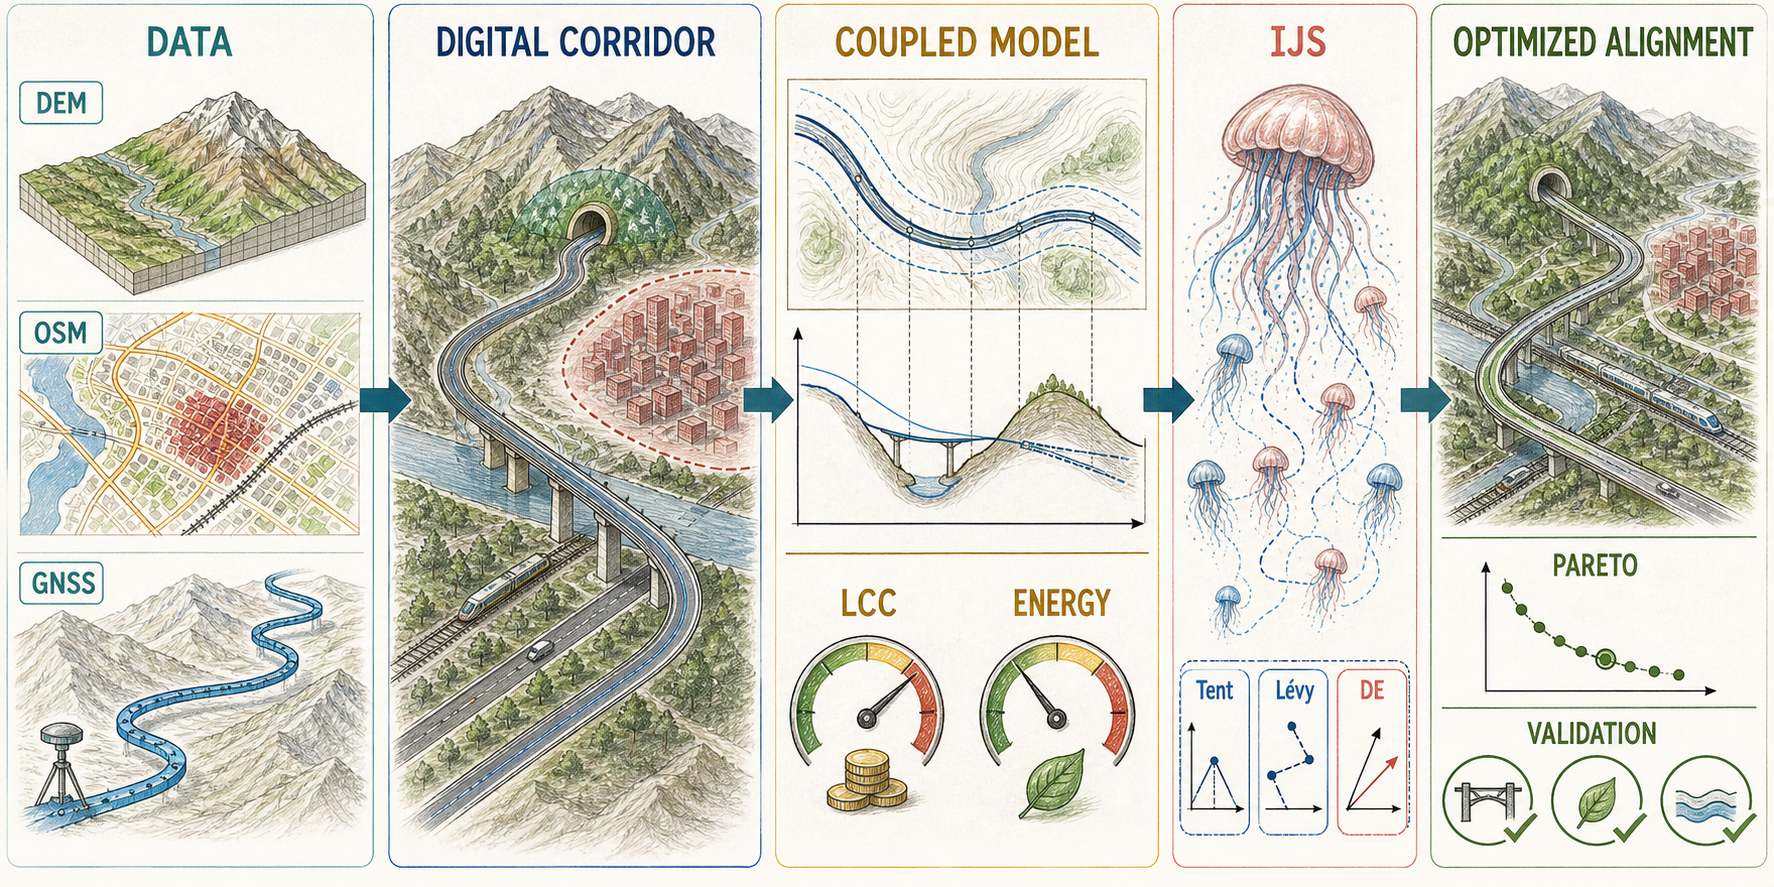
\includegraphics[width=\textwidth]{method_overview_handdrawn.png}
\caption{Data-driven workflow for collaborative three-dimensional highway alignment optimization. The hand-drawn scientific illustration highlights the information flow; the mathematical definitions are given in Sections~\ref{sec:model} and \ref{sec:solver}.}
\label{fig:overview}
\end{figure*}

\section{Related research}

\subsection{Three-dimensional alignment optimization}

Early simultaneous models demonstrated that horizontal and vertical decisions should not be optimized independently \cite{chew1989}. Evolutionary encoding subsequently made non-convex three-dimensional search practical \cite{jong2003}. GIS-based studies expanded the feasible region and allowed environmental layers to influence routing \cite{kang2012,davey2017}. Corridor-constrained horizontal search \cite{mondal2015} and rigorous vertical-alignment formulations \cite{akhmet2022} improved mathematical tractability, while bi-objective road and railway models incorporated cost, hazard and ecological impacts \cite{hirpa2016,zhang2020,song2022}.

Recent end-to-end models integrate BIM or intelligent path planners, while newer hybrid schemes combine policy optimization with population-based search \cite{han2023,pu2024,pu2026}. These methods improve automation but do not eliminate the need for transparent engineering accounting. In particular, a spatial intersection must lead to a structure or clearance decision, terrain sampling must follow the candidate line, and existing network connections must be preserved. This paper therefore prioritizes traceable geometry-to-cost mappings over an opaque surrogate objective.

\subsection{Life-cycle cost and traffic energy}

The underlying life-cycle model follows the categories in Lin \cite{lin2025}: land acquisition, bridges/tunnels, road works, maintenance and earthwork. Vehicle operation is relevant because geometric consistency affects emissions and energy demand \cite{llopis2019}. Electric-vehicle energy is especially sensitive to grade, mass, auxiliaries and regenerative behavior \cite{dimartino2022}. Rather than adding fuel and electricity in incompatible physical units, the present framework monetizes both over the analysis period. This does not claim that money is a complete environmental metric; it supplies a consistent decision scale while physical fuel and electricity components remain reportable.

\subsection{Optimization algorithms and objective decision}

NSGA-II remains a standard multi-objective benchmark \cite{deb2002}, but direct evolutionary search becomes expensive as the number of profile variables increases. Jellyfish Search models ocean-current and active/passive motion \cite{chou2021}. The present IJS adds three complementary mechanisms: a Tent map for initial coverage, L\'evy flights for non-local exploration and differential evolution (DE) for vector-wise refinement \cite{storn1997}. Section~\ref{sec:ablation} reports historical same-generation exploratory associations for these mechanisms; confirmation on the current formulation requires equal-NFE reruns.

Entropy weighting is based on the information concept of Shannon \cite{shannon1948}. Here it is applied only after feasibility and non-dominance screening. Thus a high weight cannot compensate for a geometric violation, and an infeasible solution cannot be selected merely because its cost is low.

\section{Data-driven mathematical formulation}\label{sec:model}

\subsection{Study corridor and data fusion}

The case is the Xunfengzhou--Huangcun portion of Guangzhou North Ring Expressway, a two-way six-lane urban expressway with a measured centerline length of 22.462 km. The input comprises 14,018 GNSS points with plan coordinates and elevations. These points define the existing scheme M-A, the fixed plan endpoints and the vertical tie-in elevations.

Terrain is sampled from AWS Terrain Tiles \cite{awsterrain}. Sixty zoom-level-14 tiles are decoded at approximately 8.8 m pixel spacing. Because the available surface represents the built road, a $\pm60$-m road mask is removed and interpolated from neighboring terrain to obtain a quasi-natural ground. Its correlation with the measured centerline elevation is 0.915 after a constant vertical-datum correction. This reconstruction is imperfect but applies the same terrain accounting to the existing and optimized alternatives.

OSM \cite{haklay2008,osmlicense} supplies roads, railways, watercourses and building footprints. After removing the North Ring Expressway and parallel facilities, the obstacle set contains 4,807 road features, 857 railway features and 338 river/canal features. Building footprints are rasterized on a 25-m grid and smoothed with a 200-m kernel. Thresholds are calibrated against the maximum density already traversed by M-A: Tier 2 is a hard exclusion, Tier 1 is passable with a soft discouragement, and Tier 0 is unrestricted. Figure~\ref{fig:case} shows the aligned layers.

\begin{figure*}[t]
\centering

\includegraphics[width=\textwidth]{case_data_layers.png}
\caption{Case-study data layers in the local engineering coordinate system: DEM, OSM buildings, roads, railways, watercourses, measured centerline and a displayed $\pm500$-m context band. In the optimizer $W$ is the first sine-mode amplitude, not a pointwise hard offset bound.}
\label{fig:case}
\end{figure*}

\subsection{Collaborative decision variables}

Let the measured plan line be $\bm r_0(s)=[x_0(s),y_0(s)]^\top$ with unit normal $\bm n(s)$, $s\in[0,L_0]$. A candidate plan is represented by a normal offset
\begin{equation}
\delta(s)=\sum_{k=1}^{50}a_k\sin\left(\frac{k\pi s}{L_0}\right), \qquad
|a_k|\leq \frac{W}{k^2},
\label{eq:sine}
\end{equation}
where $W=500$ m in the main experiment and $\bm r(s)=\bm r_0(s)+\delta(s)\bm n(s)$. The sine basis fixes both endpoints and attenuates high-frequency curvature. It implies the conservative spectral envelope $|\delta|\leq W\sum_{k=1}^{50}k^{-2}\approx1.625W$; hence $W$ is not a pointwise corridor boundary. The selected M-C has a maximum sampled offset of approximately 184 m. Offset control points are reconstructed by a cubic spline and evaluated on a 10-m grid. For reconstructed coordinates $(x(s),y(s))$,
\begin{equation}
\kappa(s)=\frac{|x'(s)y''(s)-y'(s)x''(s)|}
{[x'(s)^2+y'(s)^2]^{3/2}},\qquad R(s)=\kappa(s)^{-1}.
\label{eq:curvature}
\end{equation}

The vertical profile uses $M=225$ stations (approximately 100 m apart). Normalized variables generate segment grades, but the start and end design elevations $z_0$ and $z_L$ are tied to the measured road. For raw grade perturbations $h_i\in[-1,1]$, segment lengths $\Delta s_i$ and maximum grade $g_{\max}=0.04$, define
\begin{align}
\bar h&=\frac{\sum_i h_i\Delta s_i}{\sum_i\Delta s_i},\qquad
g_{\mathrm{req}}=\frac{z_L-z_0}{\sum_i\Delta s_i},\\
g_i&=g_{\mathrm{req}}+\lambda g_{\max}(h_i-\bar h),
\label{eq:grades}
\end{align}
where $\lambda\in[0,1]$ is the largest scaling that retains $|g_i|\leq g_{\max}$. Consequently $\sum_i g_i\Delta s_i=z_L-z_0$ exactly. The implementation retains a legacy start-elevation gene in its 225-slot profile block, but ignores it when $z_0$ is tied. The stored vector therefore has 275 slots and 274 referenced genes (50 modes and 224 grades). Because adding a common constant to all 224 raw grades is removed by centering, the parameterization has at most 273 locally independent degrees of freedom (50+223). This redundant direction should be eliminated before confirmatory reruns; the roughly 150 reconstruction controls are not optimization variables.

\subsection{Life-cycle cost}

The first objective is
\begin{equation}
\min C=C_R+C_B+C_S+C_Q+C_{TU},
\label{eq:lcc}
\end{equation}
where $C_R$ is land acquisition, $C_B$ bridge/tunnel cost, $C_S$ basic subgrade and pavement cost, $C_Q$ discounted maintenance and $C_{TU}$ earthwork/haulage. With road width $B$, length $L$, one mu $=666.67$ m$^2$, bridge/tunnel lengths $L_B,L_T$ and invariant ramp cost $C_{ramp}$, the implemented accounting is
\begin{align}
C_R&=c_{land}\frac{LB}{666.67}+5000\frac{L}{1000},\\
C_B&=c_B L_B+C_{ramp}+c_T L_T,\qquad
C_S=(c_{sg}+c_{pv})L,\label{eq:lccparts}\\
C_Q&=\sum_{y=1}^{T}\frac{1}{(1+r)^y}
\sum_i\Delta s_i\,[\gamma+365Q_y\tau+c_{soil}\Phi_i].
\end{align}
Here $\Phi_i$ is the weighted cut/fill slope-exposure term in the implementation; it is zero on structure-exempt segments. Unit rates follow the source thesis and the 2025 Guangzhou governmental estimation guideline \cite{guangzhou2025}. The analysis period is 30 years with a 5\% discount rate.

At station $j$, let $h_j=z_j-z^g_j$ be the design-to-ground height, $B$ the formation width and $m$ the side-slope ratio. The approximate cross-sectional earthwork area is
\begin{equation}
A_j=B|h_j|+m h_j^2.
\end{equation}
Volumes are integrated by the average-end-area method. Define the station cost rate
\begin{align}
V^{\pm}&=\sum_j\frac{A_j^{\pm}+A_{j+1}^{\pm}}{2}\Delta s_j,\\
c_j&=\begin{cases}
c_{str},& |h_j|>30\ \mathrm{m}\ \text{or}\ c_{ew}A_j>c_{str},\\
c_{ew}A_j,&\text{otherwise},
\end{cases}\\
C_{TU}&=E_L+\sum_j\frac{c_j+c_{j+1}}{2}\Delta s_j,
\label{eq:earthwork}
\end{align}
where the sign of $h_j$ selects the fill/bridge or cut/tunnel pair of rates. Structure-exempt stations have $c_j=0$. If fill/cut cost exceeds the corresponding bridge/tunnel cost, or if $|h_j|>30$ m, structural substitution is triggered. The selected structure cost replaces rather than supplements earthwork in that interval, preventing double counting and ``free floating road'' solutions.

For each candidate plan, intersections with OSM road classes primary and above, railways and watercourses trigger bridges. If $\theta_q$ is the crossing angle and $b_q$ the nominal obstacle width, the required crossing interval is
\begin{equation}
\ell_q=\frac{b_q}{\max(\sin\theta_q,\sin15^\circ)}+2E_{\mathrm{ext}},
\end{equation}
where $E_{\mathrm{ext}}=75$ m is the approach extension. Gaps under 100 m are merged. Ramp-function cost is calibrated from the seven existing interchanges and kept invariant, whereas mainline bridge length is geometric. A connected terrain region above 70 m, closed morphologically over 500 m, defines the Baiyun ecological mandatory-tunnel zone. Its area (19.2 km$^2$) and M-A crossing length (1.28 km) agree with independent project information (about 21 km$^2$ and 1.35 km, respectively).

\begin{table}[t]
\centering
\caption{Principal current-model parameters used in the case study.}
\label{tab:parameters}
\resizebox{\linewidth}{!}{\begin{tabular}{lll}
\toprule
Group & Parameter & Value \\
\midrule
Geometry & speed / width / $R_{min}$ / $g_{max}$ & 100 km/h / 25.5 m / 400 m / 4\% \\
Life cycle & $T$ / discount rate & 30 yr / 5\% \\
Land/basic works & $c_{land}$ / $c_{sg}$ / $c_{pv}$ & 58,641 RMB/mu / 200 / 30,000 RMB/m \\
Structures & $c_B$ / $c_T$ / $E_{ext}$ & 156 / 270 million RMB/km / 75 m \\
Earthwork & cut / fill / side slope & 30 / 25 RMB/m$^3$ / 1:1.5 \\
Traffic & AADT / EV share & 30,000 veh/day / 0.30 \\
Energy & fuel / electricity price & 8 RMB/L / 0.8 RMB/kWh \\
Search & population / iterations / weights & 200 / 1,000 / 21 \\
\bottomrule
\end{tabular}}
\end{table}

\subsection{Mixed fuel--electric traffic energy}

The second objective monetizes lifetime operation of a mixed fleet:
\begin{equation}
\min E=\sum_{y=1}^{30}\frac{365\,Q_y}{(1+r)^y}
\left[(1-p_{EV})c_f e_f(\bm x)+p_{EV}c_e e_e(\bm x)\right],
\label{eq:energy}
\end{equation}
where $Q_y$ is AADT, $p_{EV}=0.30$, $c_f$ and $c_e$ are fuel and electricity prices, and $e_f,e_e$ are per-vehicle route consumption. The baseline uses AADT=30,000 vehicles/day, gasoline/electricity prices of 8 RMB/L and 0.8 RMB/kWh, and the same discount rate as cost.

For a fuel vehicle, the traction load includes aerodynamic, rolling, grade and residual lateral forces. With speed $v$, mass $m_v$, aerodynamic coefficient $C_d$, frontal area $A_f$, grade angle $\alpha$ and curve radius $R$, these are
\begin{align}
F_{air}&=\tfrac12\rho C_d A_fv^2, & F_r&=C_rm_vg\cos\alpha,\\
F_g&=m_vg\sin\alpha, &
F_a&=\max\left(0,\frac{m_vv^2/R-m_vgS_p}{N_vC_s}\right).
\end{align}
For fuel vehicles the implementation converts external load to horsepower and fuel volume as
\begin{align}
P_{ex,i}&=\max\left(0,\frac{(F_{air}+F_r+F_g+F_a)v}{736\eta_f}\right),\\
e_f(\bm x)&=\sum_i \phi(HP_{in}+P_{ex,i})\frac{\Delta s_i}{v}\,/1000,
\label{eq:fuel}
\end{align}
where $e_f$ is L/vehicle-trip, $\phi=0.03$ ml/(s hp), $HP_{in}=27$ hp and $\eta_f=0.85$. The printed $10^{-3}$ multiplier in the source expression for $F_a$ is omitted: retaining it makes lateral resistance roughly five orders too small and removes the plan-curvature energy channel. This dimensional correction is explicitly disclosed rather than silently absorbed into calibration.

Electric consumption uses signed segment work $W_i=(F_{air}+F_r+F_g+F_a)\Delta s_i$:
\begin{equation}
e_e(\bm x)=\left[\frac{1}{3.6\times10^6}\sum_i
\begin{cases}W_i/\eta_e,&W_i\geq0,\\W_i\eta_e,&W_i<0,\end{cases}
\right]_+ +0.15L_{km},
\label{eq:ev}
\end{equation}
where $[x]_+=\max(x,0)$ and $\eta_e=0.90\times0.95$. Fuel and electric use are retained separately before monetary aggregation. The current main experiment evaluates a representative travel direction; fixing both endpoint elevations removes the former net-downhill bookkeeping exploit. A bidirectional mean is identified as a required extension in Section~\ref{sec:limitations}.

\subsection{Constraints and decision rule}

The hard engineering set includes fixed plan/profile endpoints, $R(s)\geq400$ m for 100 km/h design speed, $|g_i|\leq4\%$, $|g_{i+1}-g_i|\leq3\times10^{-4}\Delta s_{ctrl}$, crossing skew angle $\theta\geq15^\circ$, and zero Tier-2 penetration. Values follow JTG D20-2017 \cite{jtgd20} where directly applicable. $W$ controls sine-mode amplitudes but is not a pointwise corridor constraint; the selected current line remains inside the displayed $\pm500$-m context band. Local violations use the sum of mean and maximum relative violation, so a short severe defect cannot disappear in a long route average.

For any relative-violation vector $\bm v$, define $H(\bm v)=\operatorname{mean}(\bm v)+\max(\bm v)$. The implemented penalty is
\begin{equation}
P=\rho_t\{30H(\bm v_R)+10H(\bm v_{\Delta g})
+10H(\bm v_{skew})+10H(\bm v_{D2})\},
\label{eq:penalty}
\end{equation}
where $v_R=[400-R]_+/400$, $v_{\Delta g}$ and $v_{skew}$ are normalized excesses, and $v_{D2}=\min(d_{D2}/100,5)$. The schedule is $\rho_t=0.3$ in the first half and 3.0 thereafter. Tier 1 is deliberately excluded from $P$ and appears only as the soft term in Eq.~\eqref{eq:scalar}.

For objectives $C$ and $E$, a common baseline population supplies reference scales $C_{ref}$ and $E_{ref}$. Entropy weights $w_C,w_E$ produce
\begin{equation}
F(\bm x)=w_C\frac{C(\bm x)}{C_{ref}}+w_E\frac{E(\bm x)}{E_{ref}}
+P(\bm x)+0.22\frac{L_{T1}(\bm x)}{L(\bm x)}.
\label{eq:scalar}
\end{equation}
For an $n\times2$ objective matrix, min--max normalized entries $z_{ij}$ give $p_{ij}=z_{ij}/\sum_i z_{ij}$, entropy $e_j=-(\ln n)^{-1}\sum_i p_{ij}\ln(p_{ij}+10^{-12})$, and $w_j=(1-e_j)/\sum_k(1-e_k)$. Weights computed from a common initial population define the search scalarization. They are recomputed on the surviving front for the final compromise; these are two distinct uses of entropy weighting.

IJS solves 21 independent weighted-sum problems, so the resulting set is a weighted-sum Pareto approximation and can miss unsupported points on a non-convex front. The final decision is selected by four gates: hard feasibility, project-screening budget $C\leq1.1C_{M-A}$, non-dominance, and entropy-weighted compromise. The 10\% budget margin is an explicit planning assumption rather than a statutory threshold; its decision sensitivity remains to be tested.

\section{Improved Jellyfish Search}\label{sec:solver}

\subsection{Mechanisms}

The original JS alternates an ocean-current update toward the best solution with active/passive movement within the population \cite{chou2021}. The IJS implementation adds:

\begin{itemize}[leftmargin=*]
\item \textbf{Independent Tent initialization.} Each individual uses an independent chaotic chain with $\mu=1.99$. The exact value $\mu=2$ is avoided because finite-precision binary arithmetic collapses to zero; a single shared chain is avoided because it creates correlated individuals.
\item \textbf{Domain-scaled L\'evy flight.} The heavy-tailed perturbation is scaled by $0.01(\bm u-\bm l)$. The former unscaled implementation had only a 0.48\% acceptance rate because a unit step is not meaningful across heterogeneous variable ranges.
\item \textbf{DE refinement.} Mutation and crossover with $CR=0.5$ form a trial vector from population differences, followed by elitist acceptance \cite{storn1997}.
\end{itemize}

For reproducibility, the time control is $A_r=(1-t/T)(2u-1)$. If $|A_r|\geq0.5$, the main trial is $\bm x_i+\bm u\odot(\bm x_{best}-3u\bar{\bm x})$; otherwise the code applies active motion toward a fitter random peer or passive motion $\bm x_i+0.1\bm u\odot(\bm u_b-\bm l_b)$. The L\'evy trial is
\begin{equation}
\bm x_i^L=\bm x_i+\bm u\odot[0.01(\bm u_b-\bm l_b)\odot \bm L_{1.5}],
\end{equation}
and the DE trial uses $\bm m_i=\bm x_i+u(\bm x_{r1}-\bm x_{r2})$, binomial crossover with $CR=0.5$, and greedy replacement. Out-of-bound coordinates are reflected across the opposite bound and then clipped. Every main, L\'evy and DE trial is evaluated before elitist acceptance.

Each IJS generation therefore has about three population-equivalent evaluation phases; this is reported rather than comparing equal generation counts as equal effort. A two-phase penalty schedule uses 0.3 of the nominal penalty in the first half and 3.0 in the second half, allowing exploration near feasibility boundaries before final constraint recovery. Figure~\ref{fig:flow} gives the full process.

\begin{figure}[t]
\centering

\includegraphics[height=.72\textheight,keepaspectratio]{ijs_flowchart_handdrawn.png}
\caption{IJS solution and decision flow. Each operator is followed by elitist acceptance; the stopping branch proceeds to Pareto screening and entropy-weighted compromise selection, not geometric knee selection.}
\label{fig:flow}
\end{figure}
\FloatBarrier

\subsection{Experimental protocol}

The scheme experiment uses population 200, 1,000 IJS iterations and 21 Pareto weights (a later visual sweep uses 40). Objectives are evaluated at approximately 10-m spacing. The baseline, cost-only and joint alternatives use the same data and reference scales.

The historical ablation fixes the measured plan and uses a nominal 225-variable free-elevation profile model. Five variants (JS, +Tent, +L\'evy, +DE and complete IJS) have 30 runs, population 200 and 500 iterations. The historical benchmark compares IJS, JS, NSGA-II, real-coded GA, PSO and GWO at six profile spacings (95--500 stored variables), with 10 seeds per pair. Reported $p$ values come from independent-sample Mann--Whitney/rank-sum tests, not paired signed-rank tests. These experiments predate endpoint anchoring and density tiers. Equal generations also imply unequal NFE: approximately 100,200 for JS, 200,200 for one-added-operator variants and 300,400 for full IJS in the 500-generation ablation. They are therefore retained only as transparent development evidence and cannot establish equal-budget superiority of IJS for the current model. The same boundary applies to the 237 historical re-optimization sensitivity points.

\section{Results}

\subsection{Current engineering scheme}

Table~\ref{tab:current} and Figure~\ref{fig:scheme} report the current main result: $W=500$ m, density constraints active and endpoint elevations anchored. M-C reduces $C$ by 8.33\% and $E$ by 3.00\%. The route is 12 m longer (+0.05\%), demonstrating that the saving is not an artificial consequence of a shorter path. Bridge/tunnel cost decreases by 237 million RMB, while earthwork rises by 15 million RMB. The net effect is physically interpretable: the optimizer accepts more earthwork and a slightly longer route to reduce structural exposure and operating energy.

The reported diagnostic slope-hazard index is $Q=\sum_{u=1}^{5}W_uS_u$ with scores $S_u\in\{1,3,5\}$ and weights $(0.30,0.15,0.20,0.20,0.15)$ for topography, gully density, rainfall, geology and vegetation. The topographic score is the worse of grade-angle and cut/fill-height classes; the other four are corridor-level calibrated constants. Hence $Q$ is a comparative screening diagnostic, not a probabilistic slope-failure model or an optimization objective.

\begin{table}[t]
\centering
\caption{Current endpoint-anchored, density-constrained result.}
\label{tab:current}
\begin{threeparttable}
\begin{tabular}{lrrr}
\toprule
Metric & M-A existing & M-C optimized & Change \\
\midrule
Life-cycle cost ($10^8$ RMB) & 26.4061 & 24.2078 & $-8.33\%$ \\
Traffic energy ($10^8$ RMB) & 13.9460 & 13.5278 & $-3.00\%$ \\
\quad Fuel component & 11.1072 & 10.7911 & $-2.85\%$ \\
\quad Electricity component & 2.8388 & 2.7367 & $-3.60\%$ \\
Length (km) & 22.4618 & 22.4741 & $+0.05\%$ \\
Minimum radius (m) & 422 & 421 & feasible \\
Slope-hazard index & 3.309 & 3.298 & $-0.35\%$ \\
Tier-1 exposure (km) & 2.010 & 1.591 & $-20.85\%$ \\
Tier-2 exposure (km) & 0 & 0 & feasible \\
Penalty & 0 & 0 & feasible \\
\bottomrule
\end{tabular}
\begin{tablenotes}\footnotesize
\item Cost and energy are 30-year discounted monetary quantities. Tier-1 is passable with a soft term; Tier-2 is forbidden.
\end{tablenotes}
\end{threeparttable}
\end{table}

\begin{figure*}[t]
\centering

\includegraphics[width=\textwidth]{current_scheme_summary.pdf}
\caption{Current M-A/M-C comparison: (a) plan, (b) endpoint-anchored profile, (c) life-cycle cost decomposition and (d) headline changes. The increased earthwork and small length increase are shown explicitly.}
\label{fig:scheme}
\end{figure*}

The selected line crosses 1.591 km of Tier 1 and no Tier 2. Figure~\ref{fig:density} verifies this against the density field. It also avoids treating the existing route as an exception: Tier thresholds are calibrated so that a density already traversed by M-A is evidence of passability, while denser connected cores remain forbidden.

\begin{figure*}[t]
\centering
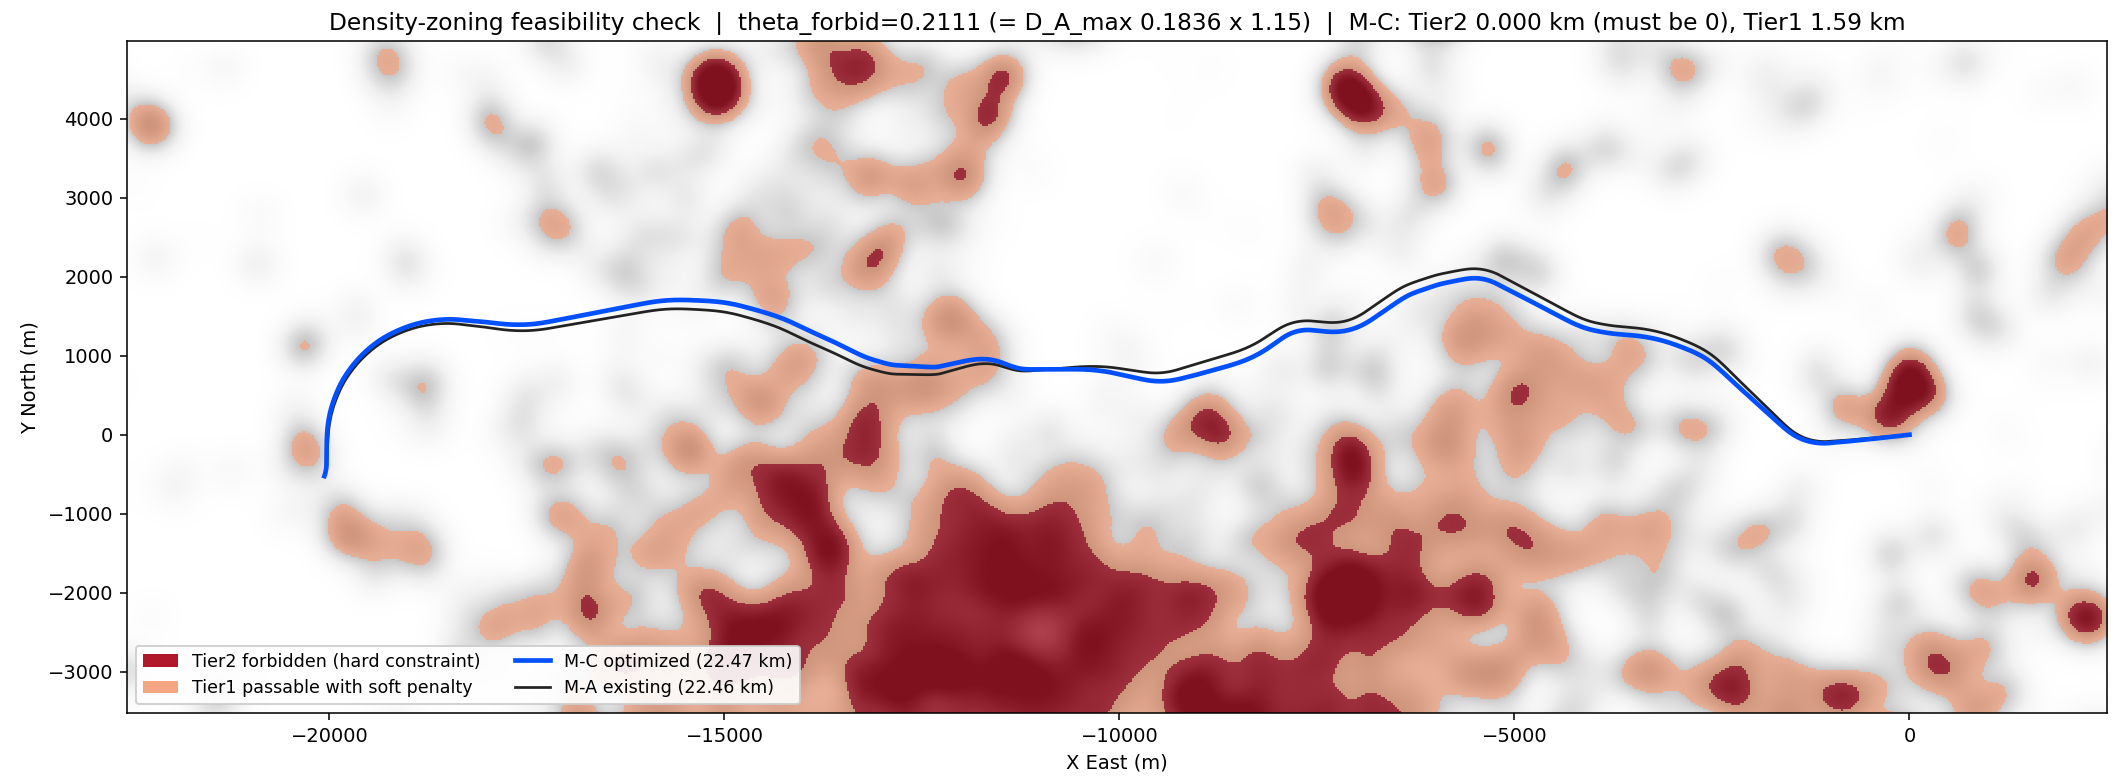
\includegraphics[width=\textwidth]{density_feasibility_w500.png}
\caption{Building-density feasibility check. The current M-C line avoids Tier-2 cores and reduces Tier-1 exposure to 1.59 km.}
\label{fig:density}
\end{figure*}

The current Pareto set (Figure~\ref{fig:pareto}) contains costly structure-heavy energy endpoints as well as the practically relevant cluster. Feasibility and the 10\% budget gate remove those extremes before entropy selection. The chosen M-C is therefore a constrained compromise, not simply the minimum of a globally normalized weighted sum.

\begin{figure}[t]
\centering

\includegraphics[width=\linewidth]{current_pareto_density.pdf}
\caption{Feasible and non-dominated screening under the current endpoint and density constraints.}
\label{fig:pareto}
\end{figure}

Figure~\ref{fig:3d} provides the spatial interpretation. The present M-C contains approximately 4.08 km of OSM-triggered crossing bridges and 0.75 km in the Baiyun ecological tunnel zone. These values differ from earlier repository figures because the current density-constrained solution is used here.

\begin{figure*}[t]
\centering

\includegraphics[width=\textwidth]{current_alignment_3d.pdf}
\caption{Current M-C on the quasi-natural DEM. At-grade, OSM-triggered bridge and ecological-tunnel intervals are distinguished; M-A is shown as a dashed reference.}
\label{fig:3d}
\end{figure*}
\FloatBarrier

\subsection{Historical pre-density control: exploratory evidence}

A controlled experiment completed before endpoint anchoring and density tiers used identical objective references and equal evaluation budgets for joint and two-stage methods. The existing line had $C=26.4061$, $E=13.9460$. The two-stage method obtained $C=23.1582$ and $E=13.4569$, apparently better than the joint result ($C=24.2239$, $E=13.4766$). However, its minimum radius was 397 m and penalty $7.36\times10^{-2}$, whereas the joint solution had 401 m and zero penalty. The lower two-stage objectives are therefore not admissible evidence of superiority. Freezing the plan after stage one removed degrees of freedom needed near the curvature boundary. This historical result motivates collaborative search, but must be rerun with current endpoint/density constraints before it can quantify a current-model effect.

\subsection{Historical same-generation IJS ablation}\label{sec:ablation}

Table~\ref{tab:ablation} shows the 30-run historical ablation. At the same generation count, IJS lowers mean $F$ from 0.9133 to 0.6808 and reaches the final JS level in 187 rather than 500 generations. The observed 25.45\% gap is confounded with about three times the NFE and an earlier free-endpoint objective; it is not an equal-budget improvement estimate. DE has the largest observed isolated gap (24.17\%) but also doubles NFE. L\'evy and Tent show 3.79\% and 1.58\% gaps. The unadjusted rank-sum $p$ values are retained for audit, not confirmatory inference.

\begin{table}[t]
\centering
\caption{Historical same-generation ablation. NFE differs by variant; $p$ values are unadjusted independent-sample rank-sum tests.}
\label{tab:ablation}
\begin{tabular}{lrrrrr}
\toprule
Variant & Mean $F$ & SD & $F_{100}$ & Observed gap & $p$ \\
\midrule
JS & 0.9133 & 0.0637 & 2.547 & -- & -- \\
JS+Tent & 0.8989 & 0.0605 & 2.227 & 1.58\% & 0.464 \\
JS+L\'evy & 0.8787 & 0.0558 & 2.095 & 3.79\% & 0.0555 \\
JS+DE & 0.6926 & 0.0315 & 1.679 & 24.17\% & $3.02\times10^{-11}$ \\
IJS & \textbf{0.6808} & 0.0340 & \textbf{1.292} & \textbf{25.45\%} & $3.02\times10^{-11}$ \\
\bottomrule
\end{tabular}
\end{table}

The corresponding observed-gap and run-distribution plots are retained as supplementary audit artifacts (\texttt{figures/ablation\_contributions.pdf} and \texttt{ablation\_boxplot.pdf}) rather than promoted as current-model confirmation.

Mechanism instrumentation clarifies the historical observation. Independent Tent chains replace 132 of 200 random initial individuals. DE use is associated with about 0.018 lower $F$ in the final 100 generations, consistent with a local-refinement hypothesis but not isolating it from the additional evaluations. A pre-defined ``escape after 20 stagnant generations'' statistic is not applicable because complete IJS rarely experiences a 20-generation stagnant interval; reporting it as zero would incorrectly imply failure.

\subsection{Historical same-generation algorithm benchmark}

At equal generation counts, IJS has the lowest historical mean $F$ at all six scales (Table~\ref{tab:benchmark}). These values describe an earlier free-endpoint model and IJS uses roughly three population-equivalent evaluations per generation, so the table cannot establish equal-budget superiority. At PJ6, IJS and JS have 10/10 feasibility whereas the other four algorithms have 0/10; this feasibility pattern remains relevant as a hypothesis for a current-model, equal-NFE rerun.

\begin{table*}[t]
\centering
\caption{Historical objective mean (SD) over ten runs. Equal generations do not mean equal NFE.}
\label{tab:benchmark}
\scriptsize
\resizebox{\textwidth}{!}{\begin{tabular}{lrrrrrr}
\toprule
Algorithm & PJ1 (95) & PJ2 & PJ3 & PJ4 & PJ5 & PJ6 (500) \\
\midrule
IJS & \textbf{.6617 (.0051)} & \textbf{.5986 (.0045)} & \textbf{.7087 (.0045)} & \textbf{.7090 (.0033)} & \textbf{.7778 (.0078)} & \textbf{.8333 (.0019)} \\
JS & .6771 (.0052) & .6104 (.0049) & .7237 (.0063) & .7215 (.0066) & .7954 (.0020) & .8563 (.0060) \\
NSGA-II & .6792 (.0045) & .6240 (.0057) & .7282 (.0053) & .7287 (.0080) & .8104 (.0084) & 12.8859 (.7330) \\
GA & .7103 (.0088) & .6478 (.0171) & .7515 (.0090) & .7489 (.0071) & 5.3906 (.5481) & 25.6024 (1.0630) \\
PSO & .7023 (.0116) & .6370 (.0113) & .7436 (.0070) & .7632 (.0072) & 9.1988 (.9109) & 32.7437 (.6336) \\
GWO & .6843 (.0065) & .6194 (.0070) & .7233 (.0046) & .7276 (.0070) & 1.1104 (.0158) & 3.2157 (1.5706) \\
\bottomrule
\end{tabular}}
\end{table*}

The six-scale convergence and PJ6 distribution plots remain available as supplementary audit artifacts (\texttt{figures/algorithm\_convergence.pdf} and \texttt{algorithm\_pj6\_boxplot.pdf}). They are omitted from the main narrative because unequal NFE prevents a confirmatory visual comparison.

IJS takes about twice the wall time of one-phase competitors at PJ1--PJ5 because L\'evy and DE add evaluations. The present record therefore supports only the statement that more evaluations per generation produced lower historical $F$. A current-model comparison must cap objective calls, pre-register paired seeds, report multiplicity-adjusted tests, effect sizes and confidence intervals, and include wall time.

\subsection{Historical free-endpoint re-optimization sensitivity}

All 237 points in the historical free-endpoint model converge to feasible solutions. They do not validate robustness of the current endpoint/density formulation. Within that earlier model, traffic growth dominates the energy response; cost is comparatively robust to demand, fleet and price factors because infrastructure cost is incurred largely at construction. Raising EV penetration moderates the high-growth energy burden, while simultaneous fuel and electricity price growth increases the monetized energy objective.

The historical spectral-width parameter produces a strong then saturating cost response: in the matched re-optimization experiment, $C$ decreases from 2.568 billion RMB at $W=200$ m to 2.239 billion RMB at $W=2{,}500$ m. The benefit accelerates once the spectral search can leave the ecological-tunnel zone, then becomes limited by urban and geometric constraints. Varying bridge approach extension $E_{ext}$ from 50/75/100 m shifts $C$ to 2.281/2.355/2.474 billion RMB, whereas $E$ remains near 1.355 billion RMB. Because this experiment uses the legacy free-endpoint model, it generates hypotheses rather than demonstrating current-model robustness.

\begin{figure*}[t]
\centering
\begin{subfigure}{.78\textwidth}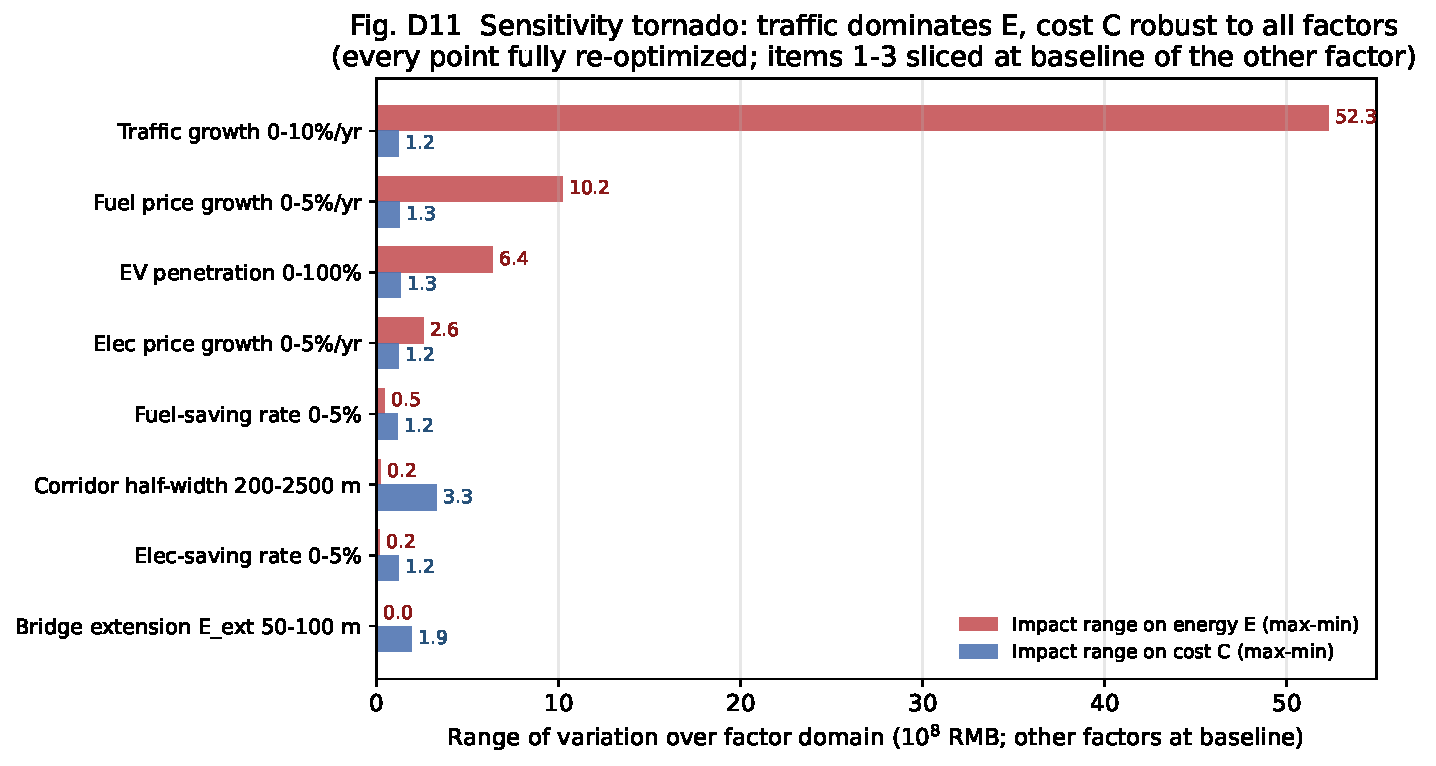
\includegraphics[width=\linewidth]{sensitivity_tornado.pdf}\caption{Relative importance of scenario factors.}\end{subfigure}\\[3mm]
\begin{subfigure}{.78\textwidth}
\includegraphics[width=\linewidth]{corridor_sensitivity.pdf}\caption{Historical spectral-width re-optimization; $W$ is not a hard geometric band.}\end{subfigure}
\caption{Historical free-endpoint sensitivity results. Every plotted point is re-optimized, but the experiment predates endpoint anchoring and density tiers.}
\label{fig:sensitivity}
\end{figure*}
\FloatBarrier

\section{Discussion}

\subsection{Engineering meaning of the improvement}

The 8.33\% cost decrease should not be interpreted as a generic saving for all expressways. It is a case-specific comparison under common data and prices. Its importance lies in the mechanism. M-C is slightly longer and has higher earthwork than M-A, but it reduces structural cost and energy while remaining outside Tier 2. The optimizer is therefore trading physical components, not merely exploiting route length. The endpoint constraints further prevent a candidate profile from receiving an unearned energy benefit by starting high and ending low.

The pre-density two-stage control illustrates why objective values alone are insufficient. Its lower $C$ and $E$ result from a line with $R_{min}=397$ m. Once feasibility is enforced, the claimed advantage disappears. Collaborative search preserves the ability to relocate horizontal crossings while reshaping the profile, which is particularly relevant where an OSM-triggered bridge and a grade transition interact.

\subsection{Role of DEM and OSM}

DEM changes the objective landscape because the ground is sampled under every candidate plan. Without it, lateral motion would affect only length and abstract land price. OSM makes structural demand and urban exposure geometry-dependent. The approach is not a substitute for survey-grade design: the dataset lacks bridge-deck elevations, parcel acquisition costs and complete building attributes. Its value is to move early-stage optimization from a one-dimensional centerline profile toward a reproducible spatial screening model.

The building tiers also clarify a policy distinction. Tier 2 is an exclusion because its density exceeds what the existing expressway demonstrates as traversable. Tier 1 is not forbidden; it carries a soft discouragement. This avoids the unrealistic claim that an urban expressway can never pass developed land while still steering alternatives away from dense clusters. In practice the soft term should be replaced by parcel-level acquisition and resettlement data.

\subsection{Algorithmic interpretation}

The historical ablation does not support a simplistic ``chaos improves everything'' narrative: Tent has the smallest observed gap and DE the largest. However, component activation also changes NFE, so the current evidence cannot separate operator quality from budget. Tent coverage, L\'evy exploration and DE refinement remain plausible mechanisms to test under objective-call stopping.

The historical benchmark suggests that feasibility should be a primary algorithmic outcome. At high resolution several competitors return penalty-dominated solutions, but whether IJS retains that advantage at equal NFE under the current formulation is unresolved. Surrogate models, parallel evaluation or decomposition are promising routes to reduce cost after a fair baseline is established.

\subsection{Limitations and validity threats}\label{sec:limitations}

The following limitations are material rather than cosmetic.

\begin{enumerate}[leftmargin=*,label=(\arabic*)]
\item The quasi-natural DEM is reconstructed by removing the present road influence, not observed before-construction terrain. Its 8.8-m pixel spacing cannot resolve local drainage and retaining structures.
\item OSM coverage is heterogeneous. Secondary roads do not trigger bridges, and bridge vertical clearance is not constrained because obstacle deck elevations are unavailable. A 15-degree skew limit is calibrated against the existing minimum of 15.6 degrees.
\item The Tier-1 weight (0.22 in normalized $F$) is a policy discouragement, not a measured demolition bill. Earlier ablation, benchmark and sensitivity experiments use both a pre-density and free-endpoint objective and unequal NFE; they are exploratory development records, not validation of the current scheme.
\item The energy objective is monetary and evaluates a representative travel direction. Endpoint anchoring removes net-elevation arbitrage, but a two-direction traffic-weighted model with calibrated regenerative braking is needed for final design.
\item Adjacent grade change is a proxy for vertical-curve smoothness. Explicit crest/sag curve lengths, non-overlap, sight distance, clothoid/arc segmentation and complete horizontal--vertical coordination checks are not yet implemented.
\item Cost rates represent early-stage estimates. Geological investigation, hydrology, parcel ownership, construction staging, embodied carbon and uncertainty are outside the current model.
\item The selected current scheme is one optimization outcome. It requires multi-seed replication; algorithm claims require equal-NFE reruns, multiplicity control, effect sizes and confidence intervals. The stored profile vector also retains one inactive legacy gene that should be removed in the next experiment release.
\end{enumerate}

These limitations define the boundary of the claim: the framework supports auditable single-run corridor screening and hypothesis generation; it does not yet support confirmatory method comparison or replace detailed geometric and construction design.

\section{Conclusions}

This study presents a data-driven, collaborative horizontal--vertical highway alignment framework that connects three-dimensional geometry to life-cycle cost and mixed fuel--electric traffic energy. The model extends an earlier mathematical base with quasi-natural DEM sampling, OSM-triggered bridges, an ecological tunnel zone, building-density tiers, structural substitution and exact endpoint tie-ins. IJS supplies the implemented candidate search process, while feasibility and non-dominance precede entropy-based decision; its comparative advantage remains a confirmatory-experiment hypothesis.

For Guangzhou North Ring Expressway, the current $W=500$-m density-constrained result reduces cost by 8.33\% and monetized energy by 3.00\%, with $R_{min}=421$ m, zero hard penalty and no Tier-2 penetration. The line is slightly longer and uses more earthwork, so the improvement is attributable to a transparent structural/operational trade rather than length alone. A two-stage historical control shows that superficially better objectives can be infeasible. Earlier ablation, benchmark and sensitivity experiments document the development path, but their free-endpoint model and unequal NFE prevent them from validating the current formulation. Equal-budget multi-seed replication is therefore a prerequisite for confirmatory algorithm claims.

The next research stage should implement bidirectional energy, survey-grade obstacle elevations, explicit vertical curves and sight distance, parcel/embodied-carbon objectives, uncertainty-aware costs and multi-seed replication of the latest density-constrained scheme. These additions would move the framework from auditable corridor planning toward design-grade decision support.

\section*{Data and code availability}
The manuscript is generated from the RoadPlan experiment repository. GNSS and project-derived files may be subject to owner restrictions; processed DEM/OSM layers, source code, fixed random seeds, result JSON files and figure-generation scripts are organized for reproducibility. The local package includes \texttt{SUPPLEMENT\_REPRODUCIBILITY.md}, a source-value snapshot and a SHA-256 manifest. A public archive and DOI should be inserted after anonymization review: \nolinkurl{[DATA-REPOSITORY-DOI-PLACEHOLDER]}.

\section*{CRediT authorship contribution statement}
\textbf{[Author name placeholders]}: Conceptualization, Methodology, Software, Validation, Investigation, Data curation, Visualization, Writing---original draft, Writing---review \& editing. Contributions must be replaced with the actual author roles before submission.

\section*{Declaration of competing interest}
The authors declare that they have no known competing financial interests or personal relationships that could have appeared to influence the work reported in this paper. This statement must be confirmed by all authors before submission.

\section*{Acknowledgements}
Funding agency, grant number and non-author contributions are intentionally anonymized and must be completed before submission.

\bibliographystyle{elsarticle-num}
\bibliography{../references}

\end{document}
